% =============================================================================
\section{Residual-Mass Bound for Stabilised Retrieval}
\label{sec:appendix_residual_bound}

The collapsed-context approximation in Section~\ref{sec:background} can be
read as a simple mixture argument.
Let $\alpha = p(c^\star \mid q)$ and define the residual context mixture
\[
  \pi_{\mathrm{res}}(r)
  =
  \frac{1}{1-\alpha}
  \sum_{c \in \mathcal{C}(q)\setminus\{c^\star\}}
  p(r \mid q,c)\,p(c\mid q),
\]
whenever $\alpha < 1$.
Then
\[
  p(r\mid q)
  =
  \alpha\,p(r\mid q,c^\star)
  +
  (1-\alpha)\,\pi_{\mathrm{res}}(r),
\]
and therefore
\[
  \bigl\|p(r\mid q)-p(r\mid q,c^\star)\bigr\|_{\mathrm{TV}}
  =
  (1-\alpha)
  \bigl\|\pi_{\mathrm{res}}(r)-p(r\mid q,c^\star)\bigr\|_{\mathrm{TV}}
  \leq 1-\alpha.
\]
The bound is not used as an estimator in the experiments.
It only states the condition under which the stylised approximation is
meaningful: the residual routing mass must be small.

% =============================================================================
\section{KG Construction and System Configuration}
\label{sec:appendix_construction}

\subsection{Knowledge Graph Construction Pipeline}
\label{sec:appendix_kg}

This section documents the full construction pipeline for reproducibility.
The key design choice is that the KG is built passage-wise with chunk-level
provenance, so every triple and path traces back to the text that licensed it.

\paragraph{Text chunking.}
Input documents are split into overlapping passages using a token-aware
recursive splitter (tiktoken-based, with a character-based fallback when the
tokenizer is unavailable) with chunk size $L = 1{,}500$ tokens and overlap
$\delta = 200$ tokens.
Each chunk receives an embedding at construction time using
\texttt{all-MiniLM-L6-v2} (384 dimensions) from Sentence Transformers
\citep{reimers2019sentencebert}.
Chunks are stored as \textsc{Chunk} nodes in Neo4j with a SHA-1 content
hash as identifier and a \textsc{Part\_Of} edge to their parent
\textsc{Document} node.

\paragraph{Entity and relation extraction.}
Entities and typed relations are extracted from each chunk via a prompted
LLM call (GPT-4o-mini; \citealp{openai2024gpt4omini}).
The LLM is prompted to return a JSON object with an \texttt{entities}
array and a \texttt{relationships} array.
Each entity has fields \texttt{id}, \texttt{type}, \texttt{name}, and
\texttt{description}; each relation has \texttt{source}, \texttt{target},
\texttt{type}, and \texttt{description}.
Two extraction modes are supported:

\begin{enumerate}
  \item \textbf{Ontology-guided extraction.} When a domain type schema is
    provided, it is first parsed from JSON or OWL/RDF into a single typed
    internal representation.
    The extraction prompt then includes ontology entity types with
    descriptions and typed properties, together with relationship types and
    their domain/range/cardinality constraints.
    After extraction, entity types are normalised with ontology guidance via
    embedding-based cosine similarity against ontology class labels
    (threshold $\tau = 0.50$), with exact substring matching and keyword
    heuristics as fallback.
    Relationship labels are then canonicalised to the closest
    schema-compatible relationship type using domain/range compatibility and
    fuzzy matching when needed.
    In the biomedical and clinical experiments, types include
    \textsc{Disease}, \textsc{Treatment}, \textsc{Symptom},
    \textsc{Biomarker}, and \textsc{Anatomy}.

  \item \textbf{Open extraction.} Without a type schema, the LLM extracts
    entities and relations freely.
    Used for the open-domain datasets (HotpotQA, HotpotQA FullWiki,
    2WikiMultiHopQA, and MuSiQue).
\end{enumerate}

The important point is that the current system does \emph{not} induce or
generate an ontology from the document collection.
It loads a user-provided ontology/schema and uses it to guide extraction,
typing, and relationship normalisation during KG construction.

\paragraph{Neo4j schema.}
Entities are stored as \textsc{Entity} nodes with compound labels
\texttt{:\_\_Entity\_\_:Type} (e.g., \texttt{:\_\_Entity\_\_:Disease}).
Each node stores an embedding vector computed from the entity name and
description.
Entities are linked to originating chunks via \textsc{Mentioned\_In} edges.
Extracted relation types (e.g., \textsc{Treats}, \textsc{Causes},
\textsc{Has\_Complication}) are stored as typed edges between entity nodes.
Three indexes are maintained: a vector index over chunk embeddings, a
vector index over entity embeddings, and a full-text keyword index over
chunk content.

\paragraph{KG scope.}
Each dataset's KG is stored as a named graph using a \texttt{kgName}
attribute on all nodes, so that multiple datasets coexist in the same
Neo4j instance without interference.
The experiment pipeline supports two build-scope modes selected by
\texttt{--dataset-kg-scope}: \textbf{evaluation\_subset} (default)
builds the KG from the same question slice being evaluated, which
minimises KG size and keeps retrieval and knowledge in the same closed
corpus; \textbf{full\_dataset} builds from all available passages in
the normalised dataset before evaluating the requested subset.
Unless explicitly noted as a diagnostic, the reported fixed-snapshot runs use
\texttt{evaluation\_subset} so that the KG and dense retriever see the same
closed corpus slice.
This improves experimental control, but it also suppresses some of the
graph-incompleteness and corpus-drift failures that would matter more in a
deployment-scale setting.

\paragraph{Relationship verification.}
After extraction, each typed relationship is verified against the chunks
that contributed at least one of its two endpoint entities (tracked via
provenance positions stored at build time).
Verification NLI is therefore run only over the source chunks, not over
the full corpus; this reduces false-positive edges from entity-name
collisions across unrelated passages.

\paragraph{Builder profiles and graph repair.}
The experiment runner exposes three KG-builder profiles:
\texttt{full}, \texttt{lightweight}, and \texttt{auto}.
Full-metrics runs use the \texttt{full} profile unless explicitly stated
otherwise.
That profile enables anchor-constrained extraction, self-reflection over
missing entities, anchor-coverage supplementation, cross-passage relation
recovery, and low-confidence triple reverification.
It also enables soft entity linking, fragmentation repair, optional graph
summaries, and claim extraction.
	For biomedical and clinical datasets the builder additionally attempts UMLS-backed
normalisation when the local SciSpaCy/UMLS stack is available; if that stack
is unavailable, construction continues without UMLS metadata rather than
failing the run.
The \texttt{lightweight} profile disables the expensive anchor, reflection,
and cross-passage extras and is reserved for quick accuracy-only sweeps.
The \texttt{auto} profile selects \texttt{lightweight} only for those cheap
question-scoped multi-hop sweeps; otherwise it resolves to \texttt{full}.

Soft linking and fragmentation repair are deliberately conservative.
The builder first canonicalises obvious aliases and near-duplicates, then
adds bridge records only for high-similarity fragments rather than freely
rewiring the graph.
Claim extraction and graph summaries are stored as additional KG artefacts;
they enrich global structure and inspection, but the eight headline
uncertainty measures reported in the main paper do not depend on them as
separate scoring heads.

\subsection{System Configuration}
\label{sec:appendix_config}

Table~\ref{tab:config} summarises the hyperparameters used across all
experiments.

\begin{table*}[t]
\centering
\small
\caption{System configuration for all experiments.
  \label{tab:config}}
\begin{tabular}{lll}
\toprule
Parameter & Vanilla RAG & KG-RAG \\
\midrule
Chunk size (tokens)           & 1,500 & 1,500 \\
Chunk overlap (tokens)        & 200   & 200   \\
Embedding model               & \multicolumn{2}{c}{\texttt{all-MiniLM-L6-v2} (384d)} \\
Top-$k$ chunks                & 10    & 10    \\
Adjacent chunk expansion      & yes (pos $\pm 1$) & -- \\
Similarity threshold          & 0.10  & 0.10  \\
Entity matching               & --    & \shortstack[l]{mention ANN ($\geq 0.72$) when query entities are extracted;\\otherwise query ANN ($\geq 0.55$); plus exact/synonym matching} \\
Chunk sufficiency threshold   & --    & 2 chunks \\
Graph scoring                 & --    & \shortstack[l]{local PPR over the retrieved entity subgraph;\\fallback to hop prior when no graph edges are available} \\
Graph expansion hops          & --    & 2 (4 for MuSiQue) \\
Iterative local hop cap      & --    & $\min(h, 3)$ per sub-question \\
Neighbours per seed entity    & --    & 30    \\
Max seed entities in prompt   & --    & 15    \\
Max neighbour entities        & --    & 10    \\
Max direct relationships      & --    & 25    \\
Iterative decomposition       & --    & enabled when the hop target is $h \geq 2$ \\
Fallback cascade              & vector & \shortstack[l]{entity-first $\to$ graph expansion $\to$ vector $\to$ text-keyword} \\
LLM (generation)              & \multicolumn{2}{c}{GPT-4o-mini} \\
Samples per question ($N$)    & \multicolumn{2}{c}{5} \\
\bottomrule
\end{tabular}
\end{table*}

\paragraph{Configuration note.}
The $k=10$ and similarity-threshold $0.10$ entries in
Table~\ref{tab:config} are the settings used by all reported runs.
The reported retrieval-study profile is \texttt{final\_pair}: vanilla RAG
is run only with the \texttt{dense\_floor} configuration, while KG-RAG is run
only with the \texttt{kg\_entity\_first} configuration.
This avoids the earlier wasteful four-way crossing of dense and graph
retrieval variants.
The strict RealMedQA mechanism ablation uses the separate
\texttt{strict\_entity} profile, which disables query fusion, late
interaction, dense fallback, vector augmentation, decomposition, and the
runtime guardrail for KG-RAG.
Iterative decomposition is also one source of retrieval variability, so
Equation~\eqref{eq:collapsed} in the main text is a stylised limit, not a
literal claim that every KG-RAG call is deterministic.
In practice, the stabilised regime is strongest on questions whose
decomposition and entity anchors converge to the same graph neighbourhood
across repeated calls.
The released manifests record the corresponding stack flags for reranking,
fallback, and query fusion, but this paper does not sweep $k$, similarity
threshold, or routing flags as independent factors.

% =============================================================================
\section{Implementation Details and Reproducibility}
\label{sec:appendix_reproducibility}

\paragraph{Question sampling.}
The codebase supports both fixed-size pilot slices and larger dataset sweeps,
and the main aggregate tables report the current fixed reported snapshot.
PubMedQA and MuSiQue retain the original fixed $n=100$ subsets.
RealMedQA is reported on its full $n=230$ evaluable question set because it is
small enough to run in full and is the main shared-corpus clinical diagnostic.
HotpotQA, HotpotQA FullWiki, and 2WikiMultiHopQA use fixed $n=250$ subsets
selected with the same seed to reduce denominator volatility in the multi-hop
analyses.
Clean-accuracy analyses can still have smaller effective denominators after
excluding provider-side generation failures, and those answered counts are
reported in the run artefacts and summarised in the main text.

For benchmark-style datasets, the current pipeline now uses deterministic
subset sampling from the full evaluable pool.
Given a dataset, sample size $n$, and subset seed $s$, it draws a fixed set
of question IDs, persists that subset on disk, and reuses the same IDs on
later runs unless a new subset is explicitly requested.
This keeps KG construction and evaluation aligned for the same
dataset/seed/sample-size combination.
Exact question IDs are stored in the run artifacts and subset manifests.

\paragraph{KG construction LLM.}
Reported KG builds use GPT-4o-mini through the configured API provider
(OpenRouter in the latest local runs) as the extraction model.
Extraction is temperature-locked at $T=0.0$ even when answer sampling uses a
higher temperature.
Biomedical and clinical datasets (PubMedQA, RealMedQA) use ontology-guided extraction
with a domain type schema (Disease, Treatment, Symptom, Biomarker, Anatomy).
Open-domain datasets (HotpotQA, HotpotQA FullWiki, 2WikiMultiHopQA, and MuSiQue) use
unconstrained open extraction.

\paragraph{Training and fine-tuning configuration.}
No task-specific model training, fine-tuning, or gradient-based calibration is
performed.
The generation model, judge model, NLI models, and embedding model are all
used as frozen off-the-shelf components.
Unless a run explicitly sets \texttt{--judge-provider} or
\texttt{--judge-model}, the correctness judge uses the same configured
GPT-4o-mini backend as answer generation.
The only learned or constructed object that changes across experiments is the
dataset-specific KG produced by the extraction pipeline.
Uncertainty samples are generated at $T=1.0$ with $N=5$ responses per
question; deterministic accuracy-generation and KG-extraction calls use
$T=0.0$.
Final-stage retrieval selection uses retrieval temperature $0.0$ in the
reported runs, with a shortlist factor of $4$ retained in the code for
stochastic retrieval sweeps.

\paragraph{NLI model.}
Discrete semantic entropy and the P(True)-style proxy cluster responses using
bidirectional NLI entailment.
All NLI inferences for DSE and the P(True)-style proxy use
\texttt{microsoft/deberta-large-mnli} \citep{he2021deberta}, run locally.
SelfCheckGPT uses \texttt{roberta-large-mnli} for pairwise contradiction
scoring.
Entailment decisions are label-based (argmax over the three-class output):
responses are placed in the same cluster when at least one direction predicts
entailment and neither direction predicts contradiction.

\paragraph{Embeddings for geometric metrics.}
VN-Entropy, SD-UQ, and SRE-UQ compute sentence embeddings of sampled
responses using \texttt{all-MiniLM-L6-v2} (384 dimensions), the same
model used for chunk and entity indexing.
Response embeddings are computed at evaluation time and are not cached.

\paragraph{Metric hyperparameters.}
GPS: maximum path length $h = 2$ hops (4 for MuSiQue), matching the
retrieval hop depth; soft answer-entity linking with
\texttt{all-MiniLM-L6-v2} cosine threshold $\tau = 0.60$ and distance decay
$\gamma = 0.4$, both selected on the RealMedQA development run over a small
grid and applied frozen to all other datasets.
Reported GPS values come from a post-hoc replay on the saved answer logs
and the persistent dataset KGs; no generation, retrieval, entity linking, or
LLM call was rerun. The run-directory replay artefacts store the linked
entities and path lengths, and the final depth-matched GPS scoring pass is
recorded under \texttt{results/analyses/}.
SD-UQ: $k_{\max} = \min(N{-}1, 8)$ principal components
(effective $k_{\max}=4$ for the reported $N=5$ samples),
$\varepsilon = 10^{-12}$.

\paragraph{Compute environment.}
All experiments were run on a MacBook Pro with an Apple~M4 chip under
macOS~15.5 (ARM64), 14 CPU cores and 52\,GB RAM, with NLI and embedding
computations on CPU.
Because KG extraction and generation use GPT-4o-mini through an API,
end-to-end wall-clock time is dominated by remote model calls: roughly
8--12 hours for the original core-suite pass, with the larger shared-corpus
and ablation runs longer (the HotpotQA FullWiki $n=250$ stress run took about
a day).
These timings are specific to the laptop-and-API setup and would likely
improve with local GPU-backed serving.

\paragraph{Effective denominators and bootstrap intervals.}
The main text reports point estimates because the analysis is organised around
family-level behaviour and qualitative traces rather than around hypothesis
tests over small AUROC gaps.
To make the scale of the evidence explicit, the appendix reports the effective
answered counts after provider-failure filtering, the usable GPS
denominators after fallback abstention filtering, and percentile-bootstrap
95\% intervals for the headline AUROCs.
All intervals below use $B=2000$ bootstrap resamples over answered questions
within each dataset and system.
For HotpotQA and 2WikiMultiHopQA in particular, the remaining GPS
denominators are small enough to make the corresponding AUROCs descriptive.

\begin{table*}[t]
\centering
\small
\caption{Summary of reported run artifacts: dataset, subset seed, sample size,
evaluation mode, and KG build scope for each reported snapshot.
All runs use GPT-4o-mini as the generation model and $N=5$ uncertainty samples.
\label{tab:run_artifacts}}
\begin{tabular}{@{}llcp{4.0cm}c@{}}
\toprule
Dataset & Subset seed & $n$ & Evaluation mode & KG build scope \\
\midrule
PubMedQA           & 42 & 100 & full\_metrics & evaluation\_subset \\
RealMedQA (adaptive) & 42 & 230 & full\_metrics & evaluation\_subset \\
RealMedQA (strict)   & 42 & 230 & full\_metrics & evaluation\_subset \\
HotpotQA           & 42 & 250 & full\_metrics & evaluation\_subset \\
HotpotQA FullWiki  & 42 & 250 & full\_metrics & evaluation\_subset \\
2WikiMultiHopQA (adaptive) & 42 & 250 & full\_metrics & evaluation\_subset \\
2WikiMultiHopQA (strict)   & 42 & 250 & full\_metrics & evaluation\_subset \\
MuSiQue            & 42 & 100 & full\_metrics & evaluation\_subset \\
\bottomrule
\end{tabular}
\end{table*}

\begin{table*}[t]
\centering
\small
\caption{Answered and failed rows in the reported saved runs.
Failures are provider- or pipeline-side generation failures and are excluded
from clean accuracy but retained in raw accounting.
The RealMedQA adaptive--strict comparison is analysed on the $196$ questions
answered by both KG policies.
\label{tab:generation_failures}}
\setlength{\tabcolsep}{4.5pt}
\begin{tabular}{@{}lrrrrrr@{}}
\toprule
Dataset & Dense ans. & Dense fail & KG ans. & KG fail & Strict ans. & Strict fail \\
\midrule
PubMedQA & 100/100 & 0 & 100/100 & 0 & -- & -- \\
RealMedQA & 219/230 & 11 & 223/230 & 7 & 200/230 & 30 \\
HotpotQA & 226/250 & 24 & 238/250 & 12 & -- & -- \\
HotpotQA FullWiki & 208/250 & 42 & 218/250 & 32 & -- & -- \\
2WikiMHQA & 212/250 & 38 & 244/250 & 6 & 245/250 & 5 \\
MuSiQue & 90/100 & 10 & 94/100 & 6 & -- & -- \\
\bottomrule
\end{tabular}
\end{table*}

\begin{table*}[t]
\centering
\small
\caption{Effective denominators for the current reported runs.
``Van answered'' and ``KG answered'' count questions remaining after
generation-failure filtering.
``GPS usable'' counts rows remaining after GPS abstention filtering.
PubMedQA and MuSiQue use fixed $n=100$ snapshots; RealMedQA uses its full
$n=230$ set; HotpotQA, HotpotQA FullWiki, and 2WikiMultiHopQA use fixed
$n=250$ snapshots.
The HotpotQA FullWiki stress snapshot is also expanded in
Table~\ref{tab:hotpot_fullwiki_stress}.
GPS columns use the final soft-linked, depth-matched estimator replayed
on the saved runs (Table~\ref{tab:realmedqa_replay} reports the corresponding
coverage before/after); RealMedQA is the GPS calibration domain.
Retrieval-state AUROC is only shown where the resulting denominator leaves an
interpretable ranking problem.
\label{tab:effective_denominators}}
\begin{tabular}{@{}lcccc@{}}
\toprule
Dataset & Van answered & KG answered & GPS usable & GPS AUROC [95\% CI] \\
\midrule
PubMedQA & 100 & 100 & -- & -- \\
RealMedQA & 219 & 223 & 195 & 0.76 [0.59, 0.90] \\
HotpotQA & 226 & 238 & 158 & 0.51 [0.42, 0.61] \\
HotpotQA FullWiki & 208 & 218 & 185 & 0.54 [0.45, 0.63] \\
2WikiMHQA & 212 & 244 & 182 & 0.38 [0.31, 0.47] \\
MuSiQue & 90 & 94 & 83 & 0.68 [0.56, 0.80] \\
\bottomrule
\end{tabular}
\end{table*}

Table~\ref{tab:gps_reliability_bins} gives a descriptive reliability view of
the same GPS scores.
The clinical calibration domain has the expected monotone shape, while several
open-domain rows do not; this is why the paper treats GPS as a conditional
graph-support diagnostic rather than a calibrated probability.

\begin{table*}[t]
\centering
\small
\caption{GPS abstention and fixed-bin empirical error rates on adaptive KG runs.  The three right columns report wrong/total rates within GPS-risk bins; lower GPS means stronger local graph support.  This is a descriptive reliability check, not an ECE calculation, because GPS is a graph-support score rather than a calibrated probability.}
\label{tab:gps_reliability_bins}
\setlength{\tabcolsep}{4pt}
\begin{tabular}{@{}lrrrrrr@{}}
\toprule
Dataset & Answered & Abstained & Usable & GPS $<.33$ & $.33$--$.67$ & GPS $>.67$ \\
\midrule
PubMedQA & 100 & 100 (100.0\%) & 0 & -- & -- & -- \\
RealMedQA & 223 & 28 (12.6\%) & 195 & 0.0\% (0/39) & 4.4\% (5/114) & 14.3\% (6/42) \\
HotpotQA & 238 & 80 (33.6\%) & 158 & 44.4\% (4/9) & 38.1\% (16/42) & 33.6\% (36/107) \\
HotpotQA FullWiki & 218 & 33 (15.1\%) & 185 & 30.0\% (21/70) & 30.8\% (16/52) & 36.5\% (23/63) \\
2WikiMHQA & 244 & 62 (25.4\%) & 182 & 33.3\% (6/18) & 50.0\% (10/20) & 27.8\% (40/144) \\
MuSiQue & 94 & 11 (11.7\%) & 83 & 33.3\% (3/9) & 50.0\% (10/20) & 70.4\% (38/54) \\
\bottomrule
\end{tabular}
\end{table*}


\begin{table*}[t]
\centering
\small
\caption{Mean pairwise retrieval-overlap summaries from the saved
reported runs.
Overlap is the mean Jaccard similarity of retrieved chunk-text sets across
the $N=5$ uncertainty-sampling calls for each question, averaged over the
run.
The current artefacts log chunk overlap at run level; they do not yet retain
per-question entity-overlap or path-overlap fields.
The strict graph-only rows are mechanism stress tests, not deployment
policies.
\label{tab:retrieval_overlap}}
\setlength{\tabcolsep}{4pt}
\begin{tabular}{@{}lcccp{5.1cm}@{}}
\toprule
Dataset & Dense & Adaptive KG & Strict KG & Reading \\
\midrule
PubMedQA & 1.000 & 0.994 & -- &
Single-abstract control; both retrievers are nearly deterministic. \\
RealMedQA & 0.952 & 0.558 & 0.661 &
Strict KG concentrates the graph context relative to adaptive KG, but dense
retrieval is also highly stable. \\
HotpotQA & 0.904 & 0.677 & -- &
Both systems retrieve stable chunk sets; the KG trace adds provenance but not
an accuracy win. \\
HotpotQA FullWiki & 0.832 & 0.516 & -- &
The shared-corpus stress run introduces more KG route and fallback variation. \\
2WikiMHQA & 0.840 & 0.802 & 0.540 &
Adaptive KG is close to dense at chunk level; strict graph-only failures are
more visible in hop-wise output collapse than in aggregate chunk overlap. \\
MuSiQue & 0.900 & 0.684 & -- &
Deep chains are stable enough for audit, but early wrong anchors still damage
answer quality. \\
\bottomrule
\end{tabular}
\end{table*}

\begin{figure*}[t]
\centering
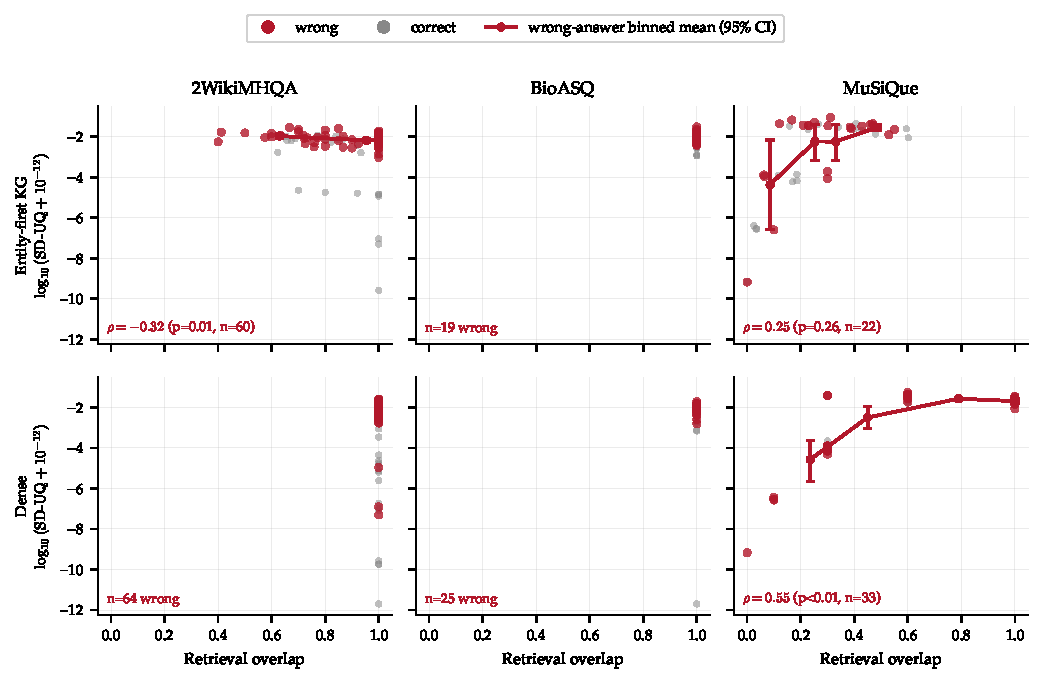
\includegraphics[width=0.92\linewidth]{figures/concentration_facets}
\caption{%
  \textbf{Full per-dataset, per-system view of the archived
  concentration--dispersion traces}, with per-dataset Spearman
  correlations among wrong answers and binned means with bootstrap $95\%$
  CIs.
  The KG-side coupling is carried by the bridge-style 2WikiMHQA trace;
  BioASQ overlap is saturated at $1.0$ (no within-dataset variation to
  correlate), and MuSiQue's small wrong set trends positive. These details keep
  the pooled $\rho=-0.27$ from being read as a between-dataset artefact or as a
  universal law.%
}
\label{fig:concentration_facets}
\end{figure*}


\begin{table*}[t]
\centering
\small
\caption{Selective risk at fixed coverage on the KG side: error rate among
the accepted questions when the most uncertain $20\%$ or $10\%$ are
abstained, using a single uncertainty signal as the gate.
``Base'' is the no-abstention error rate.
Under the adaptive policy, gating on SD-UQ alone is the strongest simple
policy; SEU gating is mediocre there because $25$--$74\%$ of adaptive rows
sit at the all-neutral $\mathrm{SEU}=0.5$ plateau, so the $80\%$ threshold
falls inside a tie mass (adaptive SEU cells are means over $200$ randomised
tie-breaking draws; the spread across draws is at most $0.006$).
Under the strict clinical ablation the ordering reverses: SD-UQ gating is no
better than accepting everything, while SEU gating removes roughly one in
five residual errors at $80\%$ coverage.
The 2WikiMultiHopQA strict run is the regime where no scalar gate helps,
consistent with the dataset-dependent survival reported in
Section~\ref{sec:results_grounding}.
\label{tab:operating_points}}
\setlength{\tabcolsep}{4pt}
\begin{tabular}{@{}lcccccc@{}}
\toprule
Run & $n$ & Base err. & SD@90\% & SD@80\% & SEU@80\% & Combined@80\% \\
\midrule
PubMedQA adaptive & 100 & 0.270 & 0.222 & 0.175 & 0.243 & 0.200 \\
RealMedQA adaptive & 223 & 0.054 & 0.030 & 0.022 & 0.054 & 0.034 \\
HotpotQA adaptive & 238 & 0.395 & 0.393 & 0.384 & 0.405 & 0.395 \\
HotpotQA FullWiki adaptive & 218 & 0.335 & 0.296 & 0.282 & 0.312 & 0.293 \\
2WikiMHQA adaptive & 244 & 0.311 & 0.282 & 0.256 & 0.261 & 0.267 \\
MuSiQue adaptive & 94 & 0.606 & 0.600 & 0.573 & 0.547 & 0.533 \\
\midrule
RealMedQA strict & 200 & 0.330 & 0.328 & 0.338 & 0.269 & 0.300 \\
2WikiMHQA strict & 245 & 0.592 & 0.600 & 0.633 & 0.668 & 0.617 \\
\bottomrule
\end{tabular}
\end{table*}

\begin{table}[t]
\centering
\small
\caption{Silent-failure sensitivity ladder: pooled fraction of wrong answers
classified as silent under progressively relaxed definitions of answer-state
dispersion.
With $N=5$ samples DSE is quantised, so $\mathrm{DSE} \leq 0.51$ admits at
most one dissenting sample (a 4-of-5 agreement gives
$\mathrm{DSE}=0.5004$).
The headline definition in Table~\ref{tab:silent_failures} is the most
conservative rung.
\label{tab:silent_sensitivity}}
\setlength{\tabcolsep}{4pt}
\begin{tabular}{@{}lccc@{}}
\toprule
Silent-error definition & Dense & Adaptive KG & Strict KG \\
\midrule
DSE $=0$ and SD-UQ at floor (headline) & 0.59 & 0.42 & 0.84 \\
DSE $=0$, any SD-UQ (unanimous)        & 0.67 & 0.52 & 0.88 \\
DSE $\leq 0.51$ ($\leq$1 dissenting sample) & 0.84 & 0.69 & 0.92 \\
\bottomrule
\end{tabular}
\end{table}

\begin{table}[t]
\centering
\small
\caption{Verbalised-confidence baseline (original P(True) protocol): the
generator backbone is asked once per saved answer for the probability that
the answer is correct, and $1-p$ is scored as uncertainty against the
paper's correctness labels.
No retrieval or generation is rerun.
AUROC treats incorrect answers as the positive class; SD-UQ columns repeat
the sampled-dispersion values for comparison.
The probe is competitive on the HotpotQA variants, weaker than SD-UQ on
RealMedQA, near chance on bridge-style 2WikiMultiHopQA under both policies,
and, unlike sampled dispersion, survives the strict clinical ablation.
\label{tab:verbalized_confidence}}
\setlength{\tabcolsep}{4.5pt}
\begin{tabular}{@{}lcc@{}}
\toprule
Run & Verbalised AUROC & SD-UQ AUROC \\
\midrule
PubMedQA adaptive & 0.55 & 0.70 \\
RealMedQA adaptive & 0.65 & 0.81 \\
HotpotQA adaptive & 0.72 & 0.64 \\
HotpotQA FullWiki adaptive & 0.77 & 0.67 \\
2WikiMHQA adaptive & 0.49 & 0.69 \\
MuSiQue adaptive & 0.65 & 0.63 \\
\midrule
RealMedQA strict & 0.89 & 0.23 \\
2WikiMHQA strict & 0.58 & 0.52 \\
\midrule
Pooled adaptive KG & 0.69 & -- \\
\bottomrule
\end{tabular}
\end{table}

\begin{table}[t]
\centering
\small
\caption{Mean marginal compute time per question for each diagnostic on the
KG side, averaged over the six headline runs (MacBook Pro M4; NLI on CPU).
Times are \emph{marginal}: they exclude the shared $N=5$ answer-sampling
calls that every answer-state estimator requires (the dominant
latency and token cost) and the cached NLI clustering shared by the
entropy-family scores.
GPS varies with graph depth (its maximum, $12.3$\,s, is the $h=4$ MuSiQue
configuration; the clinical graph costs $0.06$\,s).
\label{tab:compute_cost}}
\setlength{\tabcolsep}{5pt}
\begin{tabular}{@{}llr@{}}
\toprule
Diagnostic & Extra inputs & Mean time (s) \\
\midrule
DSE / P(True) proxy & cached NLI clusters & $<10^{-4}$ \\
SelfCheckGPT & $O(N^2)$ NLI calls & 1.68 \\
SRE-UQ & embeddings & 0.040 \\
VN-Entropy & embeddings & 0.007 \\
SD-UQ & embeddings & 0.012 \\
SEU & $K$ NLI calls & 1.65 \\
GPS & graph queries & 2.43 (0.06--12.3) \\
\bottomrule
\end{tabular}
\end{table}



\begin{table*}[t]
\centering
\small
\caption{HotpotQA FullWiki $n=250$ shared-corpus stress run.
Vanilla uses dense retrieval; KG-RAG uses the reported entity-first policy
with fallback.
Clean accuracy excludes provider-side generation failures.
GPS AUROC is reported only for KG-RAG because GPS is a graph-state diagnostic;
the GPS null rate is the fraction of answered KG rows for which the metric is
unavailable or falls back.
\label{tab:hotpot_fullwiki_stress}}
\setlength{\tabcolsep}{4pt}
\begin{tabular}{@{}lccccccccc@{}}
\toprule
Policy & Ans. & Clean acc. & Raw acc. & DSE & SRE-UQ & VN-Ent. & SD-UQ & SEU & GPS / null \\
\midrule
Dense vanilla & 208 & 0.721 & 0.600 & 0.650 & 0.630 & 0.666 & 0.665 & 0.563 & -- \\
Entity-first KG & 218 & 0.665 & 0.580 & 0.666 & 0.688 & 0.701 & 0.672 & 0.565 & 0.543 / 0.151 \\
\bottomrule
\end{tabular}
\end{table*}

\begin{table*}[t]
\centering
\small
\caption{Post-hoc RealMedQA GPS replay on the full $n=230$ answer logs.
No generation, retrieval, or LLM call was rerun; only GPS
was recomputed against the persistent dataset KG.
``Old'' is the original surface-matched, binary-reachability GPS;
``new'' is the final soft-linked, depth-matched estimator of
Section~\ref{sec:struct_metrics}.
The linking threshold and decay ($\tau=0.60$, $\gamma=0.4$) were selected on
this dataset and applied frozen everywhere else, so this table shows
calibrated in-domain behaviour; the open-domain tables provide the held-out
estimate.
\label{tab:realmedqa_replay}}
\begin{tabular}{@{}lccc@{}}
\toprule
Setting & Answered & GPS usable (old$\rightarrow$new) & GPS AUROC (old$\rightarrow$new) \\
\midrule
Dense + vanilla & 219 & 100 $\rightarrow$ 192 & 0.72 $\rightarrow$ 0.89 \\
Entity-first + KG & 223 & 97 $\rightarrow$ 195 & 0.47 $\rightarrow$ 0.76 \\
\bottomrule
\end{tabular}
\end{table*}

\begin{table*}[t]
\centering
\small
\caption{RealMedQA no-rebuild strict graph-only stress test on the full
$n=230$ question set.
The adaptive row is the reported KG policy from the full RealMedQA run.
The strict row reuses the same RealMedQA graph, disables dense fallback,
vector augmentation, and decomposition, and therefore tests whether a more
concentrated entity-first retrieval regime compresses answer-state
uncertainty.
All metric columns report AUROC.
\label{tab:realmedqa_strict_entity}}
\setlength{\tabcolsep}{3.5pt}
\begin{tabular}{@{}lcccccccc@{}}
\toprule
KG policy & Ans. & Acc. & Overlap & DSE & VN & SD-UQ & SEU & GPS \\
\midrule
Adaptive + fallback & 223 & 0.946 & 0.558 & 0.699 & 0.815 & 0.808 & 0.501 & 0.76$^\dagger$ \\
Strict graph-only & 200 & 0.670 & 0.661 & 0.463 & 0.248 & 0.233 & 0.721 & 0.746$^\dagger$ \\
\bottomrule
\end{tabular}

\vspace{0.4em}
\raggedright\footnotesize
$^\dagger$ GPS values come from the post-hoc replay
(Table~\ref{tab:realmedqa_replay}): adaptive $195/223$ usable rows, strict
$142/200$.
RealMedQA is the calibration domain for the GPS hyperparameters, so these
cells show calibrated in-domain behaviour; Table~\ref{tab:gps_reliability_bins}
gives the corresponding binned error-rate view.
\end{table*}

\paragraph{Depth-matched GPS scoring.}
GPS uses a depth-matched decay, $\gamma^{|L_e - \hat{L}|}$, where $\hat{L}$ is
the expected reasoning depth: the question's logged hop count where available
(2WikiMultiHopQA, MuSiQue), the dataset's nominal depth by construction
(HotpotQA variants, $\hat{L}=2$), and $\hat{L}=1$ otherwise.
Because $\hat{L}=1$ on RealMedQA, the calibration domain is untouched and the
frozen $(\tau, \gamma)$ carry over; all other rows are single-shot
evaluations of the same declared definition.
This is the GPS definition used in all main tables.

\begin{table*}[t]
\centering
\scriptsize
\caption{Percentile-bootstrap 95\% intervals for the headline answer-state and
evidence-state AUROCs.
These are the main answer-side metrics used in the narrative: SRE-UQ and
SD-UQ as the practical answer-state baselines, and SEU as the evidence-state signal.
The table is intended to calibrate scale, not to claim significance testing
for every pairwise gap.
\label{tab:headline_ci_output}}
\begin{tabular}{@{}lcccccc@{}}
\toprule
Dataset & SRE-UQ Van. & SRE-UQ KG & SD-UQ Van. & SD-UQ KG & SEU Van. & SEU KG \\
\midrule
PubMedQA & 0.56 [0.49, 0.64] & 0.64 [0.55, 0.73] & 0.60 [0.46, 0.74] & 0.70 [0.57, 0.81] & 0.55 [0.44, 0.67] & 0.59 [0.47, 0.71] \\
RealMedQA & 0.43 [0.24, 0.62] & 0.66 [0.51, 0.80] & 0.63 [0.39, 0.86] & 0.81 [0.64, 0.94] & 0.63 [0.47, 0.79] & 0.50 [0.35, 0.63] \\
HotpotQA & 0.61 [0.54, 0.68] & 0.63 [0.57, 0.70] & 0.64 [0.56, 0.72] & 0.64 [0.56, 0.70] & 0.46 [0.39, 0.54] & 0.48 [0.40, 0.55] \\
HotpotQA FullWiki & 0.63 [0.55, 0.71] & 0.69 [0.60, 0.76] & 0.66 [0.58, 0.75] & 0.67 [0.60, 0.75] & 0.56 [0.47, 0.65] & 0.56 [0.49, 0.64] \\
2WikiMHQA & 0.59 [0.52, 0.67] & 0.65 [0.58, 0.72] & 0.61 [0.52, 0.69] & 0.69 [0.61, 0.75] & 0.62 [0.53, 0.70] & 0.64 [0.57, 0.72] \\
MuSiQue & 0.64 [0.53, 0.75] & 0.66 [0.56, 0.77] & 0.67 [0.55, 0.78] & 0.63 [0.52, 0.75] & 0.63 [0.52, 0.75] & 0.63 [0.51, 0.74] \\
\bottomrule
\end{tabular}
\end{table*}

% =============================================================================
\section{Extended Results and Robustness Analyses}
\label{sec:appendix_extended}

This section collects secondary analyses referenced from
Section~\ref{sec:results}: silent-error threshold sensitivity, the archived
concentration--dispersion traces, the within-adaptive stability check, the
verbalised-confidence baseline, family disagreement, and the simple composite
audit score.

\subsection{Silent-Error Threshold Sensitivity}
\label{sec:appendix_silent_sensitivity}

The exact-floor silent-error definition used in
Table~\ref{tab:silent_failures} is conservative: requiring only unanimous
sampled answers (DSE $=0$, any SD-UQ) raises the pooled rates to
$52\%$/$67\%$/$88\%$ (adaptive KG / dense / strict), and admitting one
dissenting sample out of five raises them to $69\%$/$84\%$/$92\%$
(Table~\ref{tab:silent_sensitivity}), so the headline definition understates
rather than inflates the blind spot.
Unanimity at $N=5$ is already informative: if the modal answer held only
$0.7$ probability, five identical samples would occur with probability
$0.7^5 \approx 0.17$.
Two $20$-sample probes confirm the mass is not a budget artefact in the
analysed snapshots.
On the strict clinical subset, all $24$ empty-route wrong answers stay
perfectly unanimous at $N{=}20$ ($\mathrm{DSE}=0$ for every row; SD-UQ AUROC
$0.17$, unchanged from $N{=}5$).
On \emph{dense} 2WikiMultiHopQA (a pure non-graph retriever), $68\%$ of wrong
answers remain strictly silent and $86\%$ stay within one dissenting sample of
twenty, against $79\%$ strictly silent at $N{=}5$ on the headline run (the
$N{=}20$ probe uses an $n{=}100$ subset and the $N{=}5$ headline an $n{=}250$
subset, so the level at $N{=}20$ is the robust statistic rather than the
precise $79\!\to\!68\%$ delta).
Quadrupling the budget therefore barely moves the silent rate, including on
a dense system with no graph state.
These probes are deliberately narrow: they support persistence of the headline
failure mode, not a full sampling-budget sweep across every adaptive and strict
KG setting.

\subsection{Interventional Dose-Response}
\label{sec:appendix_doseresponse}

The strict-clinical collapse summarised in
Section~\ref{sec:results_collapse} is not a chunk-level stochasticity
artefact.
An interventional dose-response holds the graph, policy, prompts, and
questions fixed ($n=100$, seed 42) and varies only final-stage retrieval
determinism, sampling the final $k{=}10$ chunks from a $4k$ shortlist at
retrieval temperature $\{0, 0.5, 1.0\}$.
The manipulation works: mean within-question chunk overlap falls from
$0.67$ to $0.29$, a $57\%$ reduction. Yet the collapse does not move: SD-UQ
AUROC is $0.18/0.18/0.16$ across doses and the silent-error count is identical
($24$ of $29$--$30$ wrong, with the same $24/24$ empty-retrieval rows in each
arm).
Chunk-level stochasticity therefore does not dislodge the lock-in; the route
decomposition in Section~\ref{sec:results_collapse} locates the silent mass in
the empty-retrieval state instead.

\subsection{Archived Concentration--Dispersion Traces}
\label{sec:appendix_concentration}

Direct per-question evidence comes from three archived traces that retained
per-question retrieval overlap
(2WikiMultiHopQA $n=100$, BioASQ $n=57$, MuSiQue $n=66$;
Figure~\ref{fig:concentration_facets}).
Among \emph{wrong} KG answers the pooled coupling is negative
(Spearman $\rho = -0.27$, $p = 0.006$, $n = 101$): the more concentrated the
retrieval state, the lower the wrong-answer dispersion.
The coupling is carried by 2WikiMultiHopQA ($\rho = -0.32$, $p = 0.01$,
$n = 60$), the bridge-style dataset where lock-in is sharpest.
BioASQ's archived overlap is saturated at $1.0$, and MuSiQue's small
wrong-answer set trends the other way ($\rho = +0.25$, $n = 22$, n.s.).
On the dense side the coupling is absent where overlap is near-deterministic
and positive on MuSiQue ($\rho = +0.55$), nothing like the KG-side bridge
pattern.
These archived traces support, but do not identify, the mechanism.

\subsection{Within-Adaptive Stability Check}
\label{sec:appendix_within_stability}

An archived 2WikiMultiHopQA $n=100$ trace, unlike the newer $n=250$ run,
retained per-question chunk-overlap fields;
Table~\ref{tab:within_adaptive_stability} uses it for a small
within-adaptive sanity check.
The high-overlap band is not a monotone proof of collapse, but a useful
warning case: accuracy falls to $0.294$, DSE AUROC is near chance at $0.467$,
and VN-Entropy AUROC falls to $0.583$.
SD-UQ still carries moderate signal ($0.633$), so the result should be read
carefully.
High-stability strata thus exist inside an adaptive policy, but the logger
must persist per-question chunk, entity, and path overlap before this can be
made a headline claim.

\begin{table*}[t]
\centering
\small
\caption{%
  Within-adaptive retrieval-stability sanity check from an archived
  2WikiMultiHopQA $n=100$ trace that retained per-question chunk-overlap
  fields.  The newer $n=250$ run is the headline result; this table is a
  mechanism check.
  Bands are population tertiles of per-question chunk overlap; because a
  large fraction of questions sit at exactly $1.0$ overlap, ties spill
  across the tertile boundary.
  AUROC treats incorrect answers as the positive class.%
}
\label{tab:within_adaptive_stability}
\setlength{\tabcolsep}{3.5pt}
\begin{tabular}{@{}lrrrrrrr@{}}
\toprule
Overlap band & $n$ & Range & Acc. & DSE AUC & SD AUC & VN AUC & DSE mean \\
\midrule
Low & 33 & 0.400--0.840 & 0.364 & 0.415 & 0.714 & 0.750 & 0.277 \\
Medium & 33 & 0.850--1.000 & 0.545 & 0.667 & 0.800 & 0.752 & 0.103 \\
High & 34 & 1.000--1.000 & 0.294 & 0.467 & 0.633 & 0.583 & 0.157 \\
\bottomrule
\end{tabular}
\end{table*}


\subsection{Dedicated Per-Sample Graph-State Diversity Run}
\label{sec:appendix_diversity}

Table~\ref{tab:diversity_run} in the main text comes from a run built solely to
close the logging gap noted above: the archived traces persisted chunk overlap
alone, so the coupling could only ever be a warning case.
The diversity run was executed on HotpotQA-FullWiki ($n=221$ answered questions
with complete per-sample traces, $74$ of them wrong), reusing the existing
FullWiki knowledge graph with no rebuild, and recording for every question the
mean pairwise Jaccard overlap across the $N=5$ samples for four retrieval-state
families, namely the matched seed entities, the traversed paths, the assembled
subgraph, and the retrieved chunks, together with the per-question SD-UQ used
for the coupling test.
The two halves it confirms, a near-stable retrieval state across samples
(the premise Equation~\eqref{eq:collapsed} assumes) and a negative
overlap--dispersion coupling among wrong answers, are reported in the main
text.
The seed-entity coupling there is null only because seed overlap saturates near
$1.0$, leaving almost no variance to correlate against.
The sign and magnitude of the path, subgraph, and chunk couplings match the
archived 2WikiMultiHopQA trace of Section~\ref{sec:appendix_concentration} on
independent data and across the full set of overlap families, so the coupling no
longer rests on chunk overlap from a single archived run.

\subsection{Verbalised-Confidence Baseline}
\label{sec:appendix_verbalized}

The verbalised-confidence baseline summarised in
Section~\ref{sec:results_output} uses the original P(True) protocol, which
asks the model for a probability rather than counting cluster agreement and is
therefore not blind to silent errors by construction.
Querying the same backbone once per saved answer
(Table~\ref{tab:verbalized_confidence}) yields pooled adaptive-KG
AUROC $0.69$: competitive on the HotpotQA variants ($0.72$/$0.77$, above
SD-UQ there), weaker than SD-UQ on RealMedQA ($0.65$ vs.\ $0.81$), and near
chance precisely where bridge-style lock-in lives (2WikiMultiHopQA: $0.49$
adaptive, $0.58$ strict).
On the strict clinical ablation it reaches $0.89$ while sampled dispersion
collapses to $0.233$, so part of the clinical silent-error mass is
recoverable from the generator's own self-estimate without any retrieval-side
signal.
If a one-call self-estimate can flag clinical silent errors, why decompose at
all?
First, it fails on bridge-style lock-in
($0.49$--$0.58$), the regime the decomposition targets: where the wrong
answer is parametrically plausible, \emph{no} output-side signal tested
here, sampled or verbalised, ranks the errors.
Second, a verbalised probability is an uncalibrated self-report with known
self-preference pathologies, whereas SEU and GPS are grounded in visible
evidence and graph state.
Third, the self-estimate returns a number without a reason: when it
disagrees with the answer there is no provenance to audit, which is precisely
the evidence a clinical review workflow would need.

\subsection{Family Disagreement and the Simple Composite Audit Score}
\label{sec:appendix_composite}

\begin{figure*}[t]
\centering
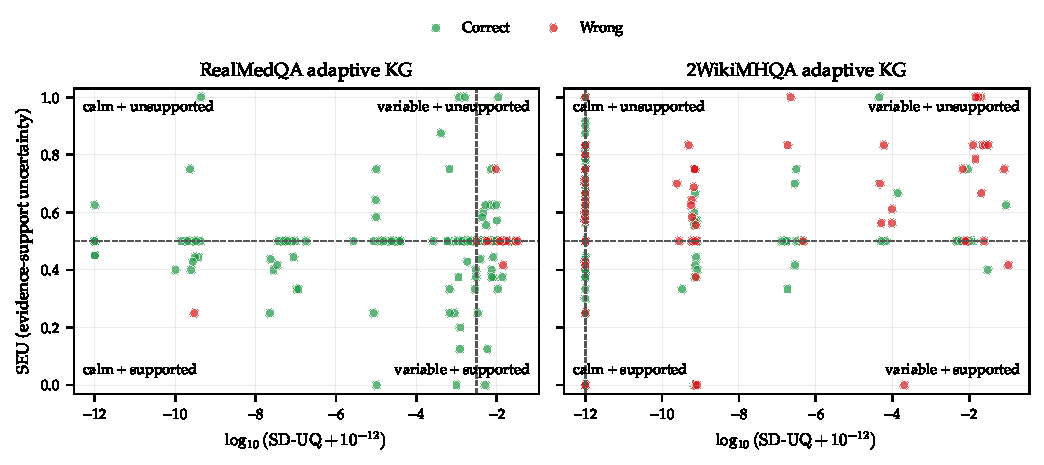
\includegraphics[width=\linewidth]{figures/family_disagreement_scatter}
\caption{%
  \textbf{Family disagreement in the pooled adaptive KG runs.}
  Grey hexagons show the density of all answered questions with a
  non-neutral SEU verdict; red points overlay the wrong answers.
  The $x$-axis is answer-state residual dispersion (SD-UQ, log scale) and
  the $y$-axis is evidence-state uncertainty (SEU).
  The all-neutral $\mathrm{SEU}=0.5$ rows, where the NLI head said nothing
  ($n=464$, $24\%$ wrong), are excluded.
  Dashed lines mark the pooled SD-UQ median and $\mathrm{SEU}=0.5$; the two
  low-answer-uncertainty quadrants carry the decision-relevant contrast:
  low answer uncertainty with contradicted evidence is $31\%$ wrong against
  $20\%$ for low answer uncertainty with support, so answer-surface agreement
  is not a proxy for evidence support.%
}
\label{fig:family_disagreement}
\end{figure*}

Beyond the conjunctive audit rule of Section~\ref{sec:results_composite},
Table~\ref{tab:composite_audit_score} gives a deliberately simple audit score:
the mean of within-dataset percentile ranks for SD-UQ, SEU, and final GPS-risk,
with GPS abstention treated as high risk.
It is uneven and not claimed to dominate the best answer-state metric.
The PubMedQA row shows where the combination earns its keep: GPS abstains on
every yes/no row (flat $0.5$), yet Combined reaches $0.813$ against SD-UQ's
$0.699$, because SEU contributes complementary support-level ranking exactly
where answer dispersion is coarse, not because the abstaining family adds
signal.
Its purpose is to show how the reported families can feed a decision layer;
a deployable policy would still need held-out calibration.

\begin{table*}[t]
\centering
\small
\caption{Adaptive-KG composite audit score.  The combined score is the mean of within-dataset percentile ranks for SD-UQ, SEU, and final GPS-risk, with GPS abstention treated as high risk.  AUROC treats incorrect answers as the positive class.  ``Base err.''\ is the no-abstention error rate; lower AUREC is better within a dataset.  ``Best single'' is the largest per-family AUROC in the row.}
\label{tab:composite_audit_score}
\setlength{\tabcolsep}{4pt}
\begin{tabular}{@{}lrrrrrrrr@{}}
\toprule
Dataset & $n$ & Base err. & SD-UQ AUC & SEU AUC & GPS-risk AUC & Best single & Combined AUC & Combined AUREC \\
\midrule
PubMedQA & 100 & 0.270 & 0.699 & 0.594 & 0.500 & 0.699 & \textbf{0.813} & 0.096 \\
RealMedQA & 223 & 0.054 & 0.808 & 0.501 & 0.703 & \textbf{0.808} & 0.729 & 0.022 \\
HotpotQA & 238 & 0.395 & 0.635 & 0.477 & 0.551 & \textbf{0.635} & 0.573 & 0.326 \\
HotpotQA FullWiki & 218 & 0.335 & 0.672 & 0.565 & 0.549 & \textbf{0.672} & 0.661 & 0.228 \\
2WikiMHQA & 244 & 0.311 & 0.685 & 0.643 & 0.414 & \textbf{0.685} & 0.619 & 0.225 \\
MuSiQue & 94 & 0.606 & 0.631 & 0.626 & 0.640 & 0.640 & \textbf{0.745} & 0.426 \\
\bottomrule
\end{tabular}
\end{table*}


\subsection{GPS Hyperparameter Sensitivity}
\label{sec:appendix_gps_sensitivity}

To test whether the headline GPS AUROCs depend on the two calibrated
hyperparameters, the soft-link threshold $\tau$ and the distance decay $\gamma$
are swept over $\tau \in \{0.50, 0.55, 0.60, 0.65, 0.70\}$ and
$\gamma \in \{0.2, 0.4, 0.6, 0.8, 1.0\}$ ($25$ cells), recomputed by offline
replay from the saved GPS replay stores. No generation, retrieval, linking, or KG
build is rerun.
Table~\ref{tab:gps_sensitivity} reports the calibrated cell (which reproduces
the headline numbers), the AUROC range across the grid, its standard deviation,
and the usable-row range.
The held-out open-domain AUROCs are robust to the hyperparameters (standard
deviation $\leq 0.018$ on HotpotQA, HotpotQA FullWiki, 2WikiMultiHopQA, and
MuSiQue), so the open-domain weakness, including the below-chance
2WikiMultiHopQA score, is a genuine retrieval limitation rather than a tuning
artefact.
The clinical calibration domain is the most sensitive ($0.038$ adaptive,
$0.091$ strict), as expected for the dataset the hyperparameters were tuned on.

\begin{table}[t]
\centering
\small
\caption{GPS AUROC sensitivity to $(\tau, \gamma)$ by offline replay.
``Calib.'' is the paper's frozen $\tau{=}0.60$, $\gamma{=}0.40$ cell; range,
SD, and usable counts are over the $5\times5$ grid.
\label{tab:gps_sensitivity}}
\setlength{\tabcolsep}{4pt}
\begin{tabular}{@{}lcccc@{}}
\toprule
Run & Calib. & Grid range & SD & Usable \\
\midrule
RealMedQA adaptive & 0.76 & 0.60--0.76 & 0.038 & 191--197 \\
RealMedQA strict   & 0.75 & 0.53--0.90 & 0.091 & 139--171 \\
HotpotQA           & 0.51 & 0.50--0.55 & 0.014 & 154--169 \\
HotpotQA FullWiki  & 0.54 & 0.53--0.56 & 0.008 & 182--187 \\
2WikiMHQA adaptive & 0.38 & 0.35--0.40 & 0.012 & 177--188 \\
2WikiMHQA strict   & 0.48 & 0.40--0.53 & 0.035 & 94--104 \\
MuSiQue            & 0.68 & 0.64--0.70 & 0.018 & 80--85 \\
\bottomrule
\end{tabular}
\end{table}

\subsection{Audit of the Fully Unflagged Residue}
\label{sec:appendix_residue}

Of the $141$ pooled adaptive-KG silent errors, $7$ ($5\%$) are unflagged by
every non-answer family (Section~\ref{sec:results_collapse}): not on an empty route,
$\mathrm{SEU}\leq 0.5$, and GPS defined and $\leq 0.5$.
A manual audit of all seven from the saved logs (question, gold answer,
generated answer) characterises them as two benchmark-ambiguous or
contested-label questions (e.g.\ the founding year of an institution with a
disputed predecessor date; a subjective ``more known for'' comparison), two
wrong-answer-slot errors where the model returns a question anchor rather than
the asked attribute (e.g.\ naming a song's performer instead of their cause of
death), and three parametric conflations or specificity mismatches (e.g.\
returning a film character's love interest instead of the lead actress's real
spouse).
SEU sits at its neutral $0.5$ default on four of the seven and below it on the
other three, so it abstains or mildly supports rather than flagging by
construction none exceed $0.5$.
Crucially, retrieved chunk texts are not archived, so none can be confirmed as
deep presence lock-in whose evidence \emph{entails} the wrong answer; the
residue is therefore better read as a mixture of label ambiguity, answer-slot
errors, and parametric overconfidence than as a wall of undetectable lock-in.

\subsection{Relocated Diagnostic Tables}
\label{sec:appendix_relocated}

Two diagnostic tables referenced from the main text are collected here to keep
the results flow tight.
Table~\ref{tab:failure_modes} summarises, per family, the regime each
diagnostic detects and where it goes silent.
Table~\ref{tab:twowiki_hopwise_diagnostics} gives the full hop-stratified
2WikiMultiHopQA comparison across the three retrieval policies; its decisive
row, the strict graph-only 4-hop slice with zero clean accuracy and collapsed
SD-UQ and VN-Entropy, is discussed in Section~\ref{sec:results_collapse}.
The table uses clean answered rows rather than raw hop-bucket sizes, so $n$
differs across policies when provider failures or skipped systems remove
rows, the same convention used for clean accuracy.

% Figure: Diagnostic behaviour across retrieval regimes.
% Full-width matrix. Include with: % Figure: Diagnostic behaviour across retrieval regimes.
% Full-width matrix. Include with: % Figure: Diagnostic behaviour across retrieval regimes.
% Full-width matrix. Include with: \input{figures/metric_failure_modes}

\begin{table*}[t]
\centering
\small
\setlength{\tabcolsep}{4pt}
\renewcommand{\arraystretch}{1.25}
\begin{tabular}{@{}p{0.15\linewidth}p{0.27\linewidth}p{0.13\linewidth}p{0.11\linewidth}p{0.11\linewidth}p{0.15\linewidth}@{}}
\toprule
\textbf{Retrieval regime}
&
\textbf{State of the context}
&
\textbf{Answer-state}
&
\textbf{SEU}
&
\textbf{GPS}
&
\textbf{Reading} \\
\midrule
Anchor failure
&
Entity linking fails; system falls back to text retrieval.
&
$\sim$~variation may persist
&
$\sim$~fallback passages
&
$\oslash$~abstains
&
Absence of a graph object is itself diagnostic. \\
\addlinespace[0.25em]
Stabilised retrieval
&
Same or near-same graph neighbourhood across samples.
&
$\downarrow$~compressed
&
\checkmark~support / contradiction
&
\checkmark~consistency
&
Agreement should be read against evidence and graph. \\
\addlinespace[0.25em]
Wrong coherent anchor
&
Anchoring succeeds on the wrong neighbourhood; paths locally coherent.
&
$\downarrow$~same wrong answer repeats
&
$\sim$~can warn
&
\texttimes~supports wrong state
&
Hardest lock-in case; trace inspection needed. \\
\addlinespace[0.25em]
KG incompleteness
&
Plausible anchor, but bridges or relations missing from the graph.
&
$\sim$~fallback restores variation
&
\checkmark~if text remains
&
$\oslash$/$\sim$~reduced
&
Coverage or construction error, not decoder uncertainty. \\
\bottomrule
\end{tabular}

\caption{%
  \textbf{Expected diagnostic behaviour across KG-RAG retrieval regimes.}
  Symbols: \checkmark~informative; $\sim$~partially informative;
  $\downarrow$~compressed and potentially silent; $\oslash$~abstains;
  \texttimes~locally consistent with a wrong state.
  Each cell states what a family can observe, not a ranking;
  Table~\ref{tab:decomposition} defines the families and
  Table~\ref{tab:failure_taxonomy} gives the resulting $2{\times}2$
  taxonomy.%
}
\label{tab:failure_modes}
\end{table*}


\begin{table*}[t]
\centering
\small
\setlength{\tabcolsep}{4pt}
\renewcommand{\arraystretch}{1.25}
\begin{tabular}{@{}p{0.15\linewidth}p{0.27\linewidth}p{0.13\linewidth}p{0.11\linewidth}p{0.11\linewidth}p{0.15\linewidth}@{}}
\toprule
\textbf{Retrieval regime}
&
\textbf{State of the context}
&
\textbf{Answer-state}
&
\textbf{SEU}
&
\textbf{GPS}
&
\textbf{Reading} \\
\midrule
Anchor failure
&
Entity linking fails; system falls back to text retrieval.
&
$\sim$~variation may persist
&
$\sim$~fallback passages
&
$\oslash$~abstains
&
Absence of a graph object is itself diagnostic. \\
\addlinespace[0.25em]
Stabilised retrieval
&
Same or near-same graph neighbourhood across samples.
&
$\downarrow$~compressed
&
\checkmark~support / contradiction
&
\checkmark~consistency
&
Agreement should be read against evidence and graph. \\
\addlinespace[0.25em]
Wrong coherent anchor
&
Anchoring succeeds on the wrong neighbourhood; paths locally coherent.
&
$\downarrow$~same wrong answer repeats
&
$\sim$~can warn
&
\texttimes~supports wrong state
&
Hardest lock-in case; trace inspection needed. \\
\addlinespace[0.25em]
KG incompleteness
&
Plausible anchor, but bridges or relations missing from the graph.
&
$\sim$~fallback restores variation
&
\checkmark~if text remains
&
$\oslash$/$\sim$~reduced
&
Coverage or construction error, not decoder uncertainty. \\
\bottomrule
\end{tabular}

\caption{%
  \textbf{Expected diagnostic behaviour across KG-RAG retrieval regimes.}
  Symbols: \checkmark~informative; $\sim$~partially informative;
  $\downarrow$~compressed and potentially silent; $\oslash$~abstains;
  \texttimes~locally consistent with a wrong state.
  Each cell states what a family can observe, not a ranking;
  Table~\ref{tab:decomposition} defines the families and
  Table~\ref{tab:failure_taxonomy} gives the resulting $2{\times}2$
  taxonomy.%
}
\label{tab:failure_modes}
\end{table*}


\begin{table*}[t]
\centering
\small
\setlength{\tabcolsep}{4pt}
\renewcommand{\arraystretch}{1.25}
\begin{tabular}{@{}p{0.15\linewidth}p{0.27\linewidth}p{0.13\linewidth}p{0.11\linewidth}p{0.11\linewidth}p{0.15\linewidth}@{}}
\toprule
\textbf{Retrieval regime}
&
\textbf{State of the context}
&
\textbf{Answer-state}
&
\textbf{SEU}
&
\textbf{GPS}
&
\textbf{Reading} \\
\midrule
Anchor failure
&
Entity linking fails; system falls back to text retrieval.
&
$\sim$~variation may persist
&
$\sim$~fallback passages
&
$\oslash$~abstains
&
Absence of a graph object is itself diagnostic. \\
\addlinespace[0.25em]
Stabilised retrieval
&
Same or near-same graph neighbourhood across samples.
&
$\downarrow$~compressed
&
\checkmark~support / contradiction
&
\checkmark~consistency
&
Agreement should be read against evidence and graph. \\
\addlinespace[0.25em]
Wrong coherent anchor
&
Anchoring succeeds on the wrong neighbourhood; paths locally coherent.
&
$\downarrow$~same wrong answer repeats
&
$\sim$~can warn
&
\texttimes~supports wrong state
&
Hardest lock-in case; trace inspection needed. \\
\addlinespace[0.25em]
KG incompleteness
&
Plausible anchor, but bridges or relations missing from the graph.
&
$\sim$~fallback restores variation
&
\checkmark~if text remains
&
$\oslash$/$\sim$~reduced
&
Coverage or construction error, not decoder uncertainty. \\
\bottomrule
\end{tabular}

\caption{%
  \textbf{Expected diagnostic behaviour across KG-RAG retrieval regimes.}
  Symbols: \checkmark~informative; $\sim$~partially informative;
  $\downarrow$~compressed and potentially silent; $\oslash$~abstains;
  \texttimes~locally consistent with a wrong state.
  Each cell states what a family can observe, not a ranking;
  Table~\ref{tab:decomposition} defines the families and
  Table~\ref{tab:failure_taxonomy} gives the resulting $2{\times}2$
  taxonomy.%
}
\label{tab:failure_modes}
\end{table*}


\begin{table*}[t]
\centering
\small
\caption{%
  Hop-wise 2WikiMultiHopQA diagnostics on the same fixed $n=250$ subset.
  The table uses clean answered rows; $n_{\mathrm{w}}$ is the AUROC positive
  class.
  AUROC is omitted when a hop slice has only one correctness class.
  The $\geq$5-hop bucket contains four questions and is kept only in the
  released JSON artefact.%
}
\label{tab:twowiki_hopwise_diagnostics}
\setlength{\tabcolsep}{3.4pt}
\begin{tabular}{@{}llrrrrrrrrrr@{}}
\toprule
Policy & Hop & $n$ & $n_{\mathrm{w}}$ & Acc. & SD mean & VN mean & SEU mean &
SD AUC & VN AUC & SEU AUC & GPS AUC \\
\midrule
Dense vanilla & 2-hop & 150 & 42 & 0.720 & 0.000 & 0.092 & 0.612 & 0.615 & 0.639 & 0.615 & 0.491 \\
Dense vanilla & 4-hop & 58 & 16 & 0.724 & 0.000 & 0.198 & 0.458 & 0.628 & 0.571 & 0.656 & 0.410 \\
Adaptive KG & 2-hop & 182 & 57 & 0.687 & 0.003 & 0.191 & 0.544 & 0.702 & 0.668 & 0.611 & 0.335 \\
Adaptive KG & 4-hop & 58 & 16 & 0.724 & 0.002 & 0.248 & 0.466 & 0.600 & 0.638 & 0.646 & 0.452 \\
Strict KG & 2-hop & 183 & 83 & 0.546 & 0.003 & 0.127 & 0.569 & 0.560 & 0.680 & 0.378 & 0.353 \\
Strict KG & 4-hop & 58 & 58 & 0.000 & 0.000 & 0.000 & 0.500 & -- & -- & -- & -- \\
\bottomrule
\end{tabular}
\end{table*}


% =============================================================================
\section{Additional Qualitative Cases}
\label{sec:appendix_cases}

\begin{table*}[t]
\centering
\small
\setlength{\tabcolsep}{4pt}
\renewcommand{\arraystretch}{1.2}
\caption{%
  \textbf{Consolidated case gallery from the reported runs.}
  \texttimes{} rows are verified lock-in failures: the KG answer is wrong yet
  repeated across all samples ($\mathrm{DSE}=0$, SD-UQ at or near the floor);
  the diagnostic columns show which family, if any, still fires.
  \checkmark{} rows are KG successes on bridge questions, where the same
  retrieval stability is helpful because the path reaches the right entity
  and relation, plus one correct answer despite GPS abstention.
  The Baltic Cup row is the hardest failure: the retrieved evidence
  \emph{entails} the wrong answer, so every scalar family reports low risk and
  only the provenance trace remains auditable.
  GPS $=0.5$ denotes abstention.
  The cases are selected for illustration, not sampled; prevalence claims
  rest on Tables~\ref{tab:silent_failures} and
  \ref{tab:failure_taxonomy}, not on this gallery.%
}
\label{tab:lockin_gallery}
\begin{tabular}{@{}c>{\raggedright\arraybackslash}p{0.26\textwidth}
                  l
                  >{\raggedright\arraybackslash}p{0.22\textwidth}
                  l c c@{}}
\toprule
\textbf{KG} & \textbf{Question (dataset)} & \textbf{Gold} & \textbf{Anchor / path}
& \textbf{KG answer} & \textbf{SEU} & \textbf{GPS} \\
\midrule
\texttimes & Osireion is behind the temple of which pharaoh? (HotpotQA)
 & Seti I
 & \emph{Ramesses II} neighbourhood of the Abydos temple
 & Ramesses II & $1.00$ & $0.44$ \\
\texttimes & Who is the paternal grandfather of Uskhal Khan? (2Wiki)
 & Khutughtu Khan
 & \emph{Toghon Tem\"ur} (father, one hop; bridge skipped)
 & Toghon Tem\"ur & $0.60$ & $0.00$ \\
\texttimes & Who created Mickey Mouse's spouse? (MuSiQue)
 & Walt Disney
 & \emph{Ub Iwerks} via Mickey Mouse $\to$ creator
 & Ub Iwerks & $0.75$ & $0.00$ \\
\texttimes & Who is Ieuan ab Owain Glynd\^wr's paternal grandfather? (2Wiki)
 & Gruffudd Fychan II
 & \emph{Owain Glynd\^wr} (father, one hop; bridge skipped)
 & Owain Glynd\^wr & $0.43$ & $0.24$ \\
\texttimes & Which country skipped the 1991 Baltic Cup? (HotpotQA)
 & Belarus
 & \emph{Estonia} via Baltic Cup participants
 & Estonia & $0.00$ & $0.00$ \\
\texttimes & Are TEC-1 and Dubna 48K based on the same processor? (HotpotQA)
 & yes
 & weak graph state; no usable anchor, GPS abstains
 & no & $0.75$ & $0.50$ \\
\texttimes & 2010 population of the city popular with tourists? (MuSiQue)
 & 8.005 million
 & wrong city; only linkable answer string four hops away
 & 2{,}217 & $0.67$ & $0.94$ \\
\midrule
\checkmark & Who is the spouse of the director of \emph{Fire-Eater}? (2Wiki)
 & Pirkko Saisio
 & film $\to$ director $\to$ spouse bridge preserved
 & Pirkko Saisio & $0.60$ & $0.44$ \\
\checkmark & Who is the father of the director of \emph{The Cup} (1999)? (2Wiki)
 & Thinley Norbu
 & film $\to$ director $\to$ father bridge preserved
 & Thinley Norbu & $0.69$ & $0.35$ \\
\checkmark & Birthplace of the director of \emph{Dollar} (1938)? (2Wiki)
 & Helsingfors
 & film $\to$ director $\to$ birthplace bridge preserved
 & Helsingfors & $0.50$ & $0.60$ \\
\checkmark & Dow Jones fall at the highest US unemployment rate? (MuSiQue)
 & 54.7\%
 & chain resolved correctly; GPS still abstains
 & 54.7\% & $0.72$ & $0.50$ \\
\bottomrule
\end{tabular}
\end{table*}


Table~\ref{tab:lockin_gallery} is the canonical case gallery.
The failure rows follow the form wrong anchor $\to$ stable retrieved context
$\to$ stable wrong answer $\to$ silent answer surface, showing per case which
diagnostic family still responds; the success rows show the same retrieval
stability working as intended on 2WikiMHQA bridge questions, where the graph
preserves the intermediate entity that vanilla retrieval loses, plus one
MuSiQue chain resolved correctly despite GPS abstention.
The main text uses one path-faithfulness example
(the Osireion lock-in of Figure~\ref{fig:lockin_trace}) to keep the exposition
focused on the lock-in mechanism; the gallery provides trace evidence, not
additional leaderboard claims.
Table~\ref{tab:path_faithfulness_case} gives the full per-family audit readout
for that Osireion case (question, retrieved graph state, and the
DSE/SD-UQ/GPS/SEU verdicts), expanding the summary in
Section~\ref{sec:results_cases}.

\begin{table*}[t]
\centering
\small
\setlength{\tabcolsep}{5pt}
\renewcommand{\arraystretch}{1.2}
\caption{%
  \textbf{Path-faithfulness failure under retrieval lock-in (HotpotQA).}
  A wrong-but-graph-coherent case from the fixed-$n=250$ run.
  The retriever anchors to a strongly associated but incorrect
  Nineteenth-Dynasty pharaoh, and every sampled answer repeats it.
  Answer-state metrics are silent and GPS reports support; only SEU fires.%
}
\label{tab:path_faithfulness_case}
\begin{tabular}{@{}>{\raggedright\arraybackslash}p{0.30\textwidth}
                  >{\raggedright\arraybackslash}p{0.30\textwidth}
                  >{\raggedright\arraybackslash}p{0.33\textwidth}@{}}
\toprule
\textbf{Question and gold answer} &
\textbf{Retrieved graph state} &
\textbf{Diagnostic reading} \\
\midrule
\emph{Osireion is located to the rear of the temple named after which New
Kingdom Nineteenth Dynasty of Egypt pharaoh?}

\vspace{0.3em}
Gold answer: \emph{Seti~I}.

\vspace{0.4em}
The intended chain attributes the Great Temple of Abydos---directly in front
of the Osireion---to its builder \emph{Seti~I}.
&
The retrieved subgraph anchors instead to \emph{Ramesses~II}, the adjacent
Nineteenth-Dynasty pharaoh who completed the temple and built his own nearby:
\begin{center}
\begin{tabular}{@{}c@{}}
Osireion / Abydos temple \\
$\downarrow$ associated pharaoh \\
Ramesses~II
\end{tabular}
\end{center}

\vspace{0.3em}
The generated KG answer is therefore \emph{Ramesses~II}~(\textbf{\texttimes}),
and dense retrieval makes the same error.
The graph state is locally coherent but attached to the wrong builder.
&
All sampled KG answers repeat the same wrong entity:
\[
  \mathrm{DSE}=0,\qquad \mathrm{SD\text{-}UQ}\approx 0.
\]
Answer-state uncertainty is therefore at its floor.

\vspace{0.3em}
GPS is low ($0.44$), so it does not flag the error:
\emph{Ramesses~II} is reachable in the retrieved graph, and GPS is reported
in risk orientation, where lower means stronger graph support for the
generated answer.

\vspace{0.3em}
SEU is maximal ($1.0$): every retrieved chunk contradicts the generated
answer, the one family that fires. \\
\bottomrule
\end{tabular}
\end{table*}


% =============================================================================
\section{Prompts}
\label{sec:appendix_prompts}

All prompts used in the experiments are reproduced verbatim below.

\subsection{Correctness Judge Prompt}
\label{sec:appendix_judge_prompt}

Used to produce the binary correctness labels on which AUROC and AUREC
are computed.

\textit{System message:}
{\small\begin{verbatim}
You are a strict answer evaluator for a factoid question answering
task. Your job is to decide if a model's response is CORRECT.

Rules:
- Reply with exactly one word: 'correct' or 'incorrect'.
- The response is CORRECT only if it contains an answer semantically
  equivalent to the expected answer (minor spelling/accent differences
  are ok).
- The response is INCORRECT if the model says it doesn't know, cannot
  determine, or provides a factually different answer.
\end{verbatim}}

\textit{User message (template):}
{\small\begin{verbatim}
Question: {question}
Expected answer: {expected_answer}
Model response: {model_response}

Is the model response correct? Reply with one word only:
correct or incorrect.
\end{verbatim}}

\subsection{Vanilla RAG Generation Prompt}
\label{sec:appendix_vanilla_prompt}

Used by the vanilla RAG system to generate all $N = 5$ sampled
responses per question.

\textit{System message (template):}
{\small\begin{verbatim}
You are an AI assistant that provides accurate, factual answers
based on the provided context.

Context Information:
{context}

Guidelines:
- Read all context passages carefully -- the answer is often present
  but may require connecting two passages.
- For multi-hop questions: explicitly chain your reasoning step by
  step (e.g. "The film starred X -> X later held position Y").
- Base your answer on the provided context; do not invent facts.
- If the answer is not directly stated but can be inferred by
  connecting two pieces of evidence, make the inference explicitly
  and state your reasoning chain.
- Only say the context is insufficient if you genuinely cannot find
  any relevant evidence after carefully reading all passages.
- Be concise but comprehensive; include specific facts to support
  your answer.
- IMPORTANT: For yes/no questions (questions starting with: Is, Are,
  Does, Do, Can, Should, Was, Were, Has, Have), you MUST begin your
  response with either "Yes" or "No" as the very first word,
  followed by your explanation.

User Query: {question}
\end{verbatim}}

\subsection{KG-RAG Generation Prompt}
\label{sec:appendix_kg_prompt}

Used by the KG-RAG system to generate all $N = 5$ sampled responses
per question.
The instruction to prefer evidence appearing in \emph{both} text chunks
and graph paths is the proximate cause of consistent, confident generation
under KG context, one mechanism that amplifies graph-induced
overconfidence.

\textit{System message (template):}
{\small\begin{verbatim}
You are a knowledgeable AI assistant. Answer the question using
the provided context.

The context has three parts:

1. TEXT CHUNKS -- document passages retrieved by semantic similarity.
2. GRAPH TRAVERSAL PATHS -- multi-hop chains discovered by walking
   the knowledge graph from seed entities.
   Each path shows how concepts connect:
   Entity A --RELATIONSHIP--> Entity B --RELATIONSHIP--> Entity C
3. ENTITIES -- individual concepts found in the graph.

HOW TO REASON:
- Read all text chunks carefully -- the answer is often present but
  requires connecting two passages.
- Start from the entities most relevant to the question, then follow
  graph paths to discover indirect relationships.
- For multi-hop questions: explicitly chain your reasoning step by
  step (e.g. "The film starred X -> X later held position Y").
- Prefer evidence that appears in BOTH a text chunk AND a graph path
  -- that is the strongest signal.

IMPORTANT:
- For yes/no questions, begin with "Yes" or "No" followed by your
  explanation.
- Ground every claim in the provided context; do not invent facts.
- If the answer is not directly stated but can be inferred by
  connecting two pieces of evidence in the context, make the
  inference explicitly and state your reasoning chain.
- Only say the context is insufficient if you genuinely cannot find
  any relevant evidence after carefully reading all passages.

Text Chunks:
{context}

Knowledge Graph Traversal Paths:
{graph_paths}

Entities:
{entities}

Question: {question}
\end{verbatim}}

\subsection{Entity Extraction Prompts}

The prompts used for LLM-based entity and relation extraction during KG
construction (open and ontology-guided modes) follow the JSON schema
described in Appendix~\ref{sec:appendix_kg}.
They are available in the supplementary code release
(Appendix~\ref{sec:appendix_code}).

% =============================================================================
% =============================================================================
\section{\system{} System Description}
\label{sec:appendix_ontographrag}

\system{} (v1.0.0-rc1) is the open-source platform used to run all
reported experiments.
It exposes a FastAPI application on port 8004, started with
\texttt{uvicorn ontographrag.api.app:app --host 0.0.0.0 --port 8004}
or via the installed console script \texttt{ontograph}.
Neo4j is checked at startup; endpoints requiring the graph database
return \texttt{HTTP 503} if unavailable.

\subsection{Package Structure}

\begin{description}
  \item[\texttt{ontographrag.kg}]
    KG construction. \texttt{builders/} contains the open extraction
    and ontology-guided extraction pipelines.
    \texttt{loaders/} handles Neo4j serialisation, and \texttt{utils/}
    contains chunking, source-node, and graph-query helpers.

  \item[\texttt{ontographrag.rag}]
    \texttt{EnhancedRAGSystem} (KG-RAG pipeline) and
    \texttt{VanillaRAGSystem} (dense-retrieval baseline), with auxiliary
    modules for reranking, retrieval sampling, and answer guardrails.

  \item[\texttt{ontographrag.providers}]
    Unified LLM interface supporting OpenAI, Anthropic, Google Gemini,
    Vertex AI, OpenRouter, and Ollama.
\end{description}

Persistence: Neo4j $\geq$5.25 for all graph, vector, and full-text indexes.
Chunk and entity embeddings are stored as Neo4j native vector indexes;
no external vector store is required.
Install with \texttt{pip install .}; deployment requires Python $\geq$3.11
and Neo4j connection environment variables.

\subsection{Serving Interface}

The full REST API is documented in the accompanying software release rather
than reproduced here.
For the reported experiments, the relevant interface is the question
answering endpoint: it returns the generated answer, retrieved text chunks,
matched entities, graph paths, route labels, relation anchors, and per-query
diagnostic scores.
The manuscript therefore treats the API as infrastructure for trace logging,
not as a separate systems contribution.

% =============================================================================
\section{Code and Data Availability}
\label{sec:appendix_code}

The system implementation, the experiment harness, and the scripts that
generate every table and figure in this paper are available at
\url{https://github.com/julka01/OntoGraphRAG}.
The supplementary run artefacts are released in the same repository: the raw
per-run logs, the fixed sampled question IDs for each snapshot, both judges'
correctness labels, the raw per-query metric scores and uncertainty estimates,
and the GPS replay stores used for the post-hoc recomputations (the RealMedQA
replay, the $\tau\times\gamma$ sensitivity sweep, and the HotpotQA-FullWiki
diversity run).
The release bundle is \texttt{reproducibility/arxiv\_v1/}, and
\texttt{reproducibility/arxiv\_v1/MANIFEST.json} records the exact repository
commit and file hashes for the cached logs used in the paper.
Because every fixed-subset number and every post-hoc replay in the paper is
computed from these saved artefacts, the reported results can be reproduced
without rerunning generation or retrieval.

\paragraph{Reproducibility checklist.}
Table~\ref{tab:repro_checklist} consolidates the exact configuration values
scattered through this appendix.

\begin{table*}[t]
\centering
\small
\caption{Reproducibility checklist (verified against the released run
artefacts and code).
\label{tab:repro_checklist}}
\setlength{\tabcolsep}{5pt}
\begin{tabular}{@{}lp{9.2cm}@{}}
\toprule
Item & Value \\
\midrule
Generation model & \texttt{gpt-4o-mini} via OpenRouter (\texttt{openai/gpt-4o-mini}); $T{=}1.0$ for the $N{=}5$ uncertainty samples, $T{=}0.0$ for accuracy generation and KG extraction \\
Judge model (main) & same \texttt{gpt-4o-mini} backbone as generation \\
Judge model (re-judge) & \texttt{meta-llama/llama-3.3-70b-instruct} via OpenRouter, $T{=}0.0$ \\
Embedding model & \texttt{all-MiniLM-L6-v2} (384-d, Sentence Transformers), shared by chunks, entities, and response embeddings \\
NLI models & \texttt{microsoft/deberta-large-mnli} (DSE / P(True) clustering, SEU); \texttt{roberta-large-mnli} (SelfCheckGPT pairwise) \\
Subset seeds & $42$ for every dataset and run (including dose-response and $N{=}20$ probes) \\
Sampling budget & $N{=}5$ headline; $N{=}20$ resampling probe \\
GPS calibration and sensitivity & $\tau{=}0.60$, $\gamma{=}0.40$ selected on the RealMedQA replay and applied frozen elsewhere; Appendix~\ref{sec:appendix_gps_sensitivity} replays $\tau \in \{0.50,\ldots,0.70\}$ and $\gamma \in \{0.2,\ldots,1.0\}$ \\
Cached reproduction & headline tables and figures regenerate from released saved artefacts; no API calls, KG rebuild, or generation rerun is required for the reported analyses \\
Retrieval temperature & $0.0$ in all reported runs; $\{0, 0.5, 1.0\}$ in the dose-response arms (shortlist factor $4$) \\
Provider failures & per-run generation failures excluded from clean accuracy: KG side $0$--$32$ and dense side $0$--$42$ per run (Table~\ref{tab:generation_failures}) \\
Code version & \texttt{OntoGraphRAG} v1.0.0, public repository; exact commit and artefact hashes recorded in the released manifest \\
\bottomrule
\end{tabular}
\end{table*}

\paragraph{Mechanism-probe artefacts.}
The post-submission mechanism analyses reported in
Section~\ref{sec:results_collapse} have their own artefacts, released
alongside the run logs: the retrieval-temperature dose-response runs
(RealMedQA, strict profile, $n=100$, seed 42, retrieval temperatures
$\{0, 0.5, 1.0\}$, with per-question chunk overlap retained), the
$N{=}20$ resampling probe on the same strict subset, the independent
re-judge of all free-text runs
(\texttt{rejudge\_independent.json}, \texttt{rejudge\_wave1.json}), the
verbalised-confidence baseline (\texttt{verbalized\_confidence.json}),
the audit-rule evaluation with matched-coverage baselines and split-half
validation (\texttt{certificate\_eval.json}), the silent-rate sensitivity
and route-decomposition numbers (\texttt{wave1\_analysis.json}), the
reporting-robustness bookkeeping for failure counts and the audit rule
odds ratio (\texttt{reporting\_robustness.json}), and the
KG scale statistics queried from the persistent Neo4j stores
(\texttt{kg\_scale\_stats.json}).
